\chapter{Summary and Future Directions}\label{chap:conclusion}


Future RV missions: MINERVA \cite{minerva}, HPF
\cite{2012SPIE.8446E..1SM}, WIYN-NEID, etc.

Magellan/PFS \cite{2010SPIE.7735E..53C}


Each chapter already has its own conclusion and future works. This
chapter will summarize the main findings in this thesis, and outlining
potential future directions that are not direct extensions on the
works documented in previous chapters.

%------------------
promised to talk about limitation of the CPS code/algorithm, and the
new RV code.

The work described in the previous sections is all done with the
California Planet Search Consortium Doppler code, which is a legacy
code in IDL primarily written by John A.\ Johnson but with legacy
parts that date back to the work of Marcy \& Butler as early as
1989. It is proven to be able to produce RVs at $\sim 1$
\mps\ precision with Keck data, and is behind the discoveries and
characterization of numerous exoplanets, including the first
Earth-mass Earth-radius planet Kepler-78b \citep{howard2013,pepe2013}.

Yet, this great legacy code has many drawbacks: It is based on a
simple home-constructed Levenberg–-Marquardt least $\chi^2$ fitter
(LM fitter) which has high requirement on initial guesses for
parameters and is terribly inefficient and inadequate in exploring the
$\chi^2$ space. It also has many legacy house keeping parts and
complicated structures that makes it hard to upgrade, adopt for other
instruments, and add new modules and functions.

We have set out to write a new RV code that is built in {\it Python}.
The new code carries on the valuable successful parts of the CPS code
over, and more importantly, built to be highly modular and thus will
be easy to adopt for other instruments or to plug in modern
numerical and statistical tools.

We have completed the structural design and built the core part of the
code, where it fits one spectral chunk using any designated maximum
likelihood style fitter (e.g.\ a better LM fitter, which yield a
smaller $\chi^2_\nu$ value when testing with Keck spectral chunks). We
plan to make it fully functional for the commissioning of MINERVA in
Summer 2015 (see Section~3 for future plans to implement more
advanced tools).


{\bf (2)} I will build a next-generation Doppler pipeline for current
and next-generation RV instruments (in {\tt Python} and public on {\tt
  GitHub}). This new pipeline employs advanced statistical and
numerical tools such as Bayesian MCMC algorithm and Gaussian processes
(Figure~\ref{fig:newrv2}), which will model the correlated noise
originated from a complex blaze function, normalization issues, CCD
effects, telluric line modeling residuals, imperfect deconvolved
stellar spectrum, and so on (see, e.g., \citealt{starfish} and Daniel
Foreman-Mackey's {\it george} package). This new package is built to
be highly modular and easily adaptable to any RV
instrument. Magellan/PFS is a great instrument to implement this new
package: the upgraded PFS will have the largest pixel sampling factor
among all RV instruments, providing more modeling power for RV
extraction.

{\bf (3)} I will implement features for estimating RVs induced by
stellar activity in the new package, such as bisector fitting,
analysis on line depth change, and color-dependent RV estimate. This
will be the first time the stellar activity and planetary RV signals
are disentangled {\it directly from the spectral data}, instead of
estimating and subtracting the effects of stellar activity ``after the
fact". I will take advantage of the unique high-cadence capability of
MINERVA and obtain carefully designed RV time series on a sample of
bench-mark stars (e.g. $\tau$ Ceti and $\sigma$ Dra), thereby,
tackling the problem of stellar activity-induced RVs.


Currently there is a large cry in the RV community for a public,
high-precision RV code which would allow better transparency and cross
checking of results. We have made our code publicly available through
{\tt gitHub}, and we plan to document the methods in peer-reviewed
literature once the code is ready to be released for the greater
community.

%------------------
promised to talk about new vanking project.

% on MINERVA


% on the upgraded HET/HRS

This will also contain work on MINERVA and EPDS and looking forward to
other future work.



%----------------------------------------------------------------
% MCMC triangle plot for a Keck chunk fit
% plot from Jobs/plots/, made by newrv code and hand edited for 2015
% postdoc proposals
\begin{figure}
\centering
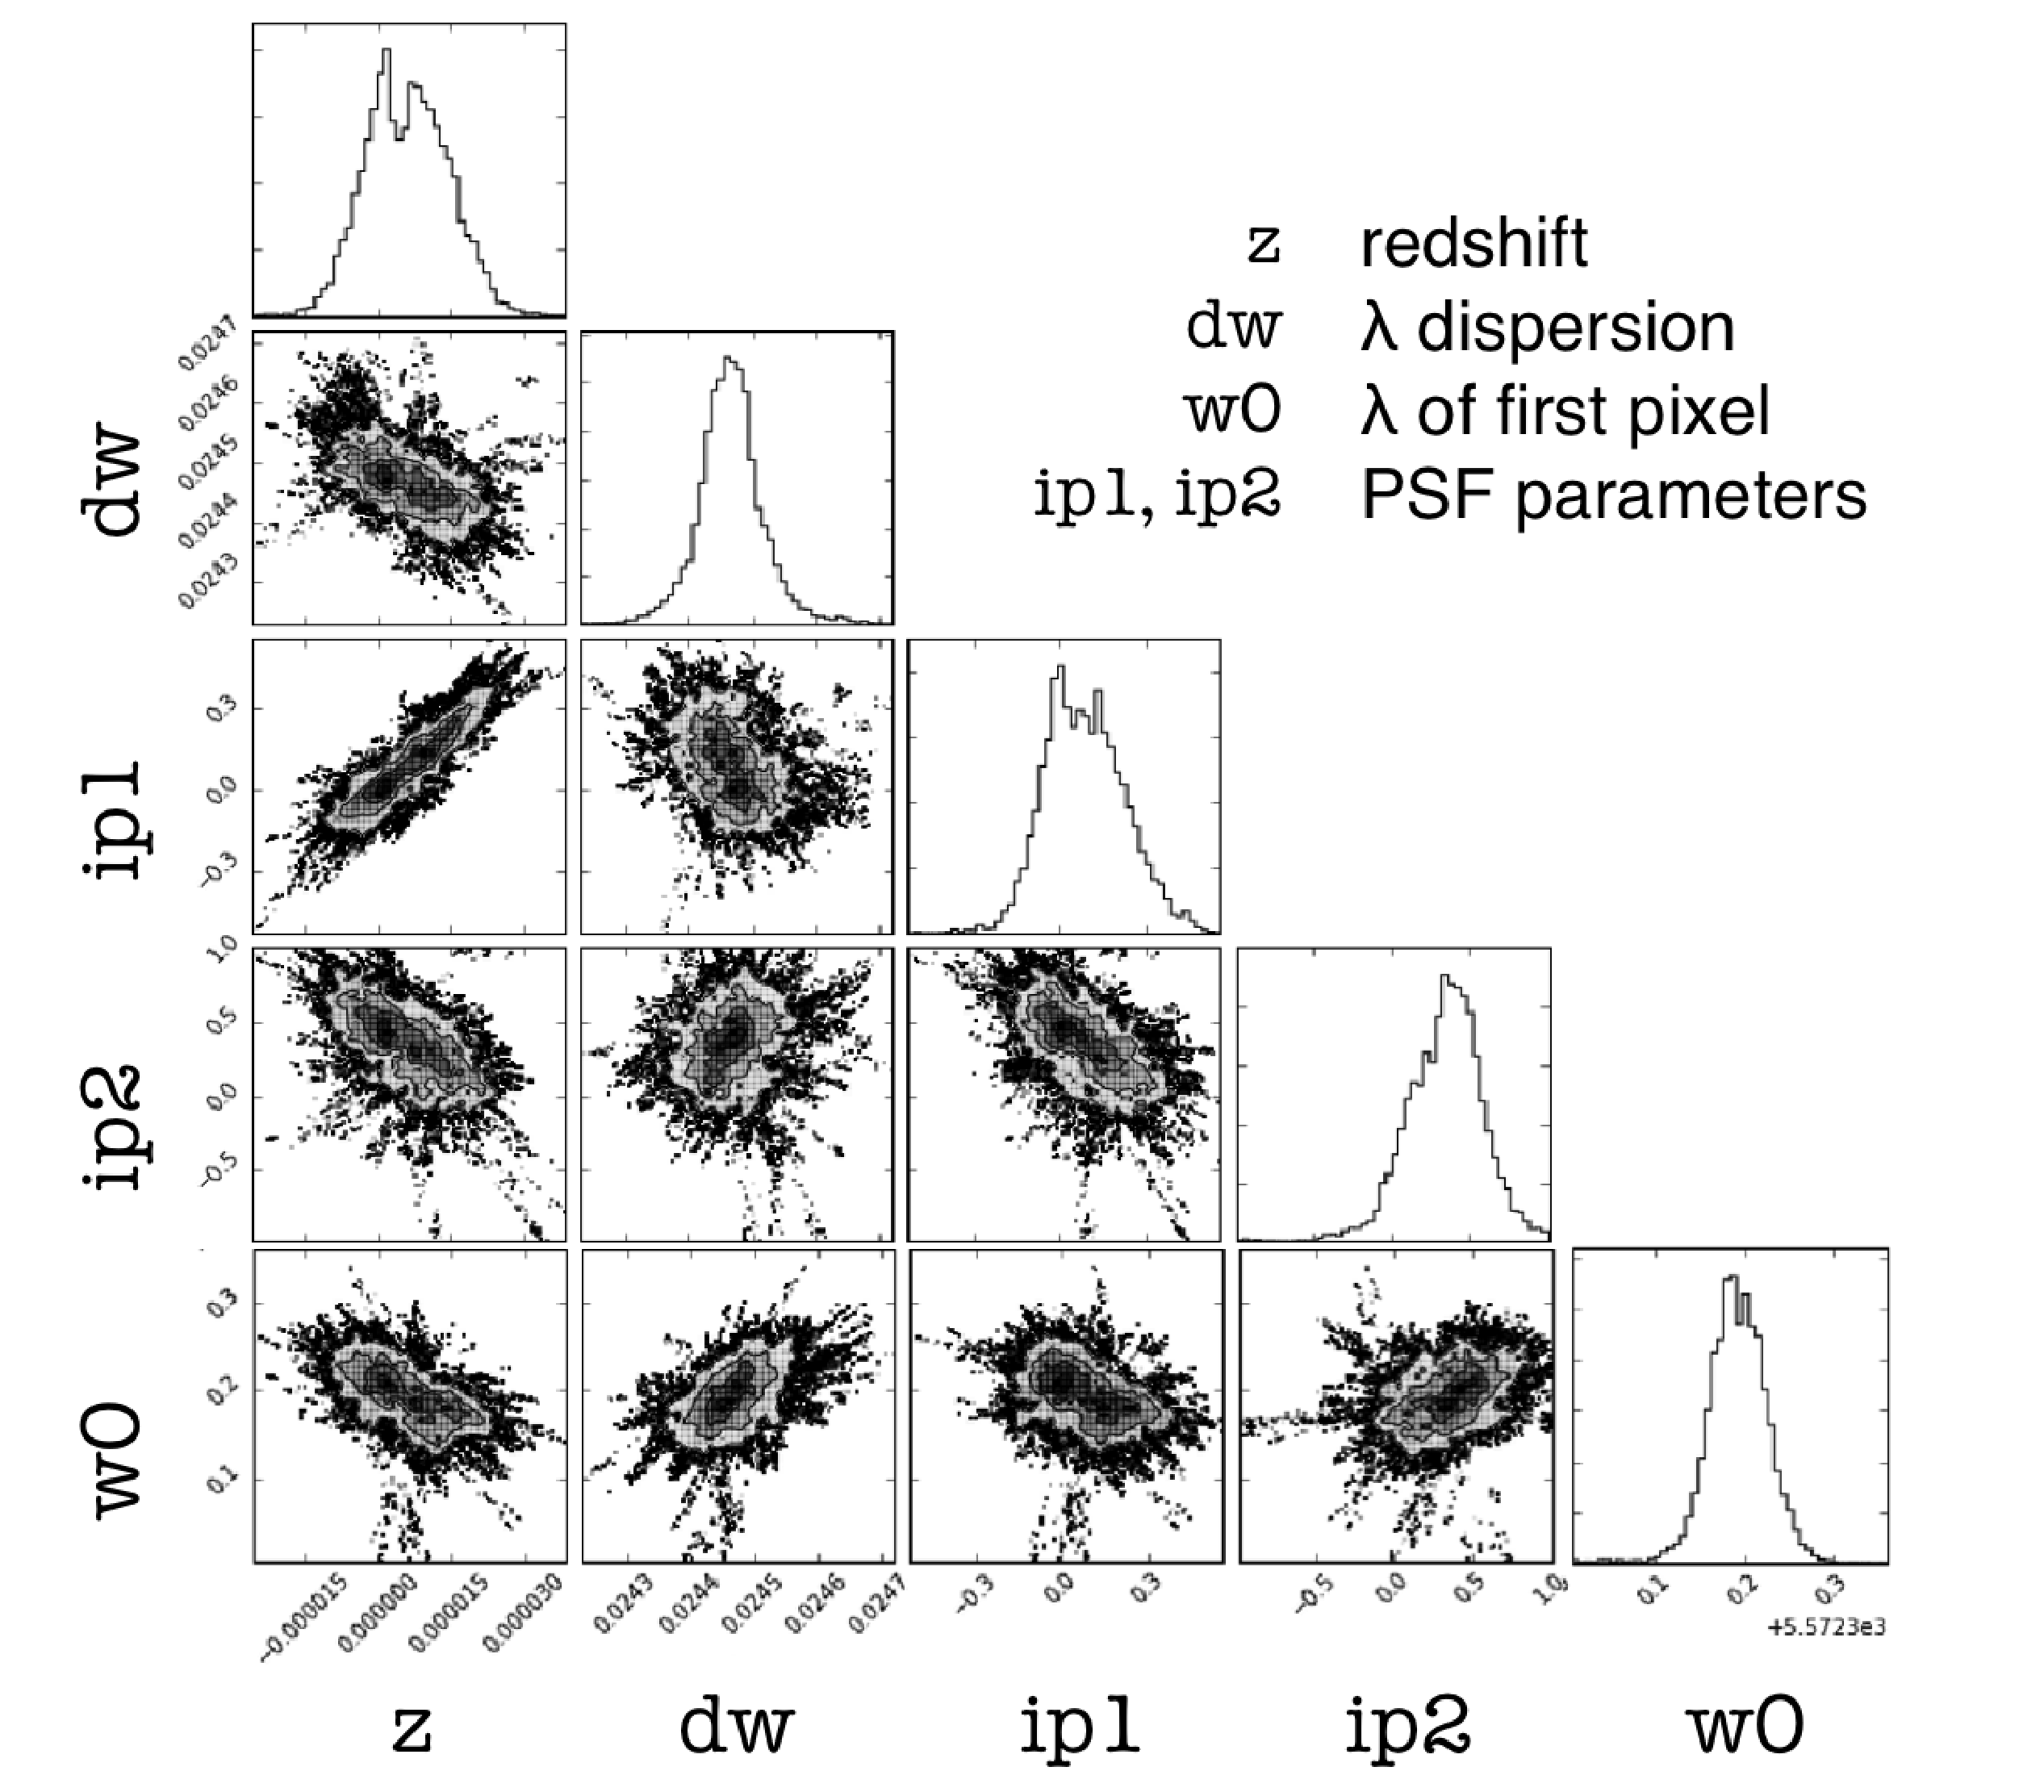
\includegraphics[scale=0.3]{conclusion/mcmcplot-labeled.eps}
\caption{Preliminary results from the new code.
\label{conclusion:fig:mcmc}}
\end{figure}
%----------------------------------------------------------------
